\documentclass{beamer}
%
% Choose how your presentation looks.
%
% For more themes, color themes and font themes, see:
% http://deic.uab.es/~iblanes/beamer_gallery/index_by_theme.html
%
\mode<presentation>
{
  \usetheme{Madrid}      % or try Darmstadt, Madrid, Warsaw, ...
  \usecolortheme{beaver} % or try albatross, beaver, crane, ...
  \usefonttheme{serif}  % or try serif, structurebold, ...
  \setbeamertemplate{navigation symbols}{}
  \setbeamertemplate{caption}[numbered]
  %%% Author/Title/Date and slide number in the footline
  \setbeamertemplate{footline}[author title date]
  %%% Puts the section/subsection in the headline
  \setbeamertemplate{headline}[section]
  
%%% Set a background colour
% \setbeamercolor{background canvas}{bg=lightgrey}
} 

\graphicspath{{./img/}}
\DeclareGraphicsExtensions{.pdf,.png,.jpg}

\usepackage[brazil]{babel}
%\usepackage[brazilian]{babel}
%\usepackage[T1]{fontenc} 
\usepackage{ae,url} 
\usepackage{amssymb,amsmath}
\usepackage[utf8]{inputenc}
\usepackage{comment} %% cc
\usepackage{listings}
\lstset{numbers=left, keepspaces=true, columns=flexible}



\title{Introdução ao Raciocínio Lógico para ALP}
\author{Rafael Alceste Berri -- \textit{rafaelberri@usp.br}\\Claudio Cesar de Sá -- \textit{claudio.sa@udesc.br}}
\institute{Universidade do Estado de Santa Catarina \\ Departamento de Ciência da Computação}
\date{\today}

% The log drawn in the upper right corner.
%\logo{\includegraphics[height=0.03\paperheight]{udesc_joinville}}

\begin{document}
\maketitle

\tableofcontents

\begin{frame}
\frametitle{Atenção ...}

\begin{exampleblock}{....}

Este texto reflete as dificuldades básicas que alunos
tiveram na disciplina de ALP em semestre anterioes.\\
 
 Todo conteúdo encontra-se sob revisão constante e está
 distante de um formato final!

\end{exampleblock}
\end{frame}




\begin{frame}
\frametitle{\textit{Aquecendo no desequilíbrio}, ou desigualdades:}

\begin{center}
 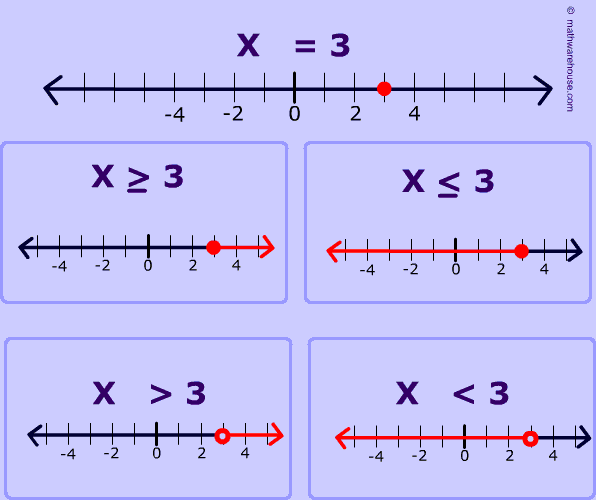
\includegraphics[height=0.6\textheight,width=0.8\textwidth]{figuras/number-line-inequality-graph-example1.png} 
\end{center}

\end{frame}




\begin{frame}
\frametitle{Refletindo sobre as inequações serão úteis:}

\begin{exampleblock}
%%{Seja $x \in N$, avalie a \textbf{verdade} das expressões:}
{Seja $x \in \{0,1..99\}$, avalie a \textbf{verdade} das expressões:}
\begin{enumerate}
  
  \item $ x > 100$
  
  \item $x$ é ímpar ou $x$ é par
  
  \item $\forall x(12x + x^2 \le 12)$

  \item $\forall x(144 \ge 12x + 7)$

  \item $\forall x(128 - 14x \le 12x + 4)$
      
      
\end{enumerate}
\end{exampleblock}
\end{frame}


\begin{frame}
\frametitle{As inequações serão úteis:}

\begin{exampleblock}
%%{Seja $x \in N$, avalie a \textbf{verdade} das expressões:}
{Seja $x \in \{0,1..99\}$, avalie a \textbf{verdade} das expressões:}
\begin{enumerate}
  
  \item $ x > 100$ \hspace{1cm} \textcolor{red}{R: 0}
  
  \item $x$ é ímpar ou $x$ é par \hspace{1cm} \textcolor{red}{R: 1}

  
  \item $\forall x(12x + x^2 \le 12)$
\hspace{1cm} \textcolor{red}{R: 0 ou falsa}



  \item $\forall x(144 \ge 12x + 7)$ 
\hspace{1cm} \textcolor{red}{R: 0 ou falsa}

  \item $\forall x(128 - 14x \le 12x + 4)$ 
\hspace{1cm} \textcolor{red}{R: 0 ou falsa}
      
\end{enumerate}
\end{exampleblock}
\end{frame}











\begin{frame}
\frametitle{Questões de concurso público, tais como:}

\begin{exampleblock}{A negação de ``\textit{hoje é domingo}"\/ é:}
\begin{enumerate}
  \item hoje é domingo
  \item hoje não é domingo
  \item hoje não, não é domingo
  \item hoje é sábado
\end{enumerate}
\end{exampleblock}

\pause
\begin{block}{A negação de ``\textit{hoje é domingo e amanhã não choverá}"\/ é:}
\begin{enumerate}
  \item hoje não é domingo e amanhã não choverá
  \item hoje não é domingo ou amanhã choverá
  \item hoje não é domingo então amanhã choverá
  \item hoje não é domingo nem amanhã choverá
\end{enumerate}
\end{block}
\pause
\begin{alertblock}{Assim ...}
precisamos de algo mais \textbf{forte}!
\end{alertblock}
\end{frame}

\begin{frame}
\frametitle{Este \textit{mais forte} é ...}

\begin{block}{}
\begin{enumerate}
  \item Transformar as frases do tipo ``\textit{hoje é domingo}" \/ em afirmações 
  (assertivas ou proposições)   
  \item Estas serão \textbf{Verdadeiras} ou \textbf{Falsas}, como nas inequações, exemplo: $2+3 > 6$
  \item Construir fórmulas a partir destas proposições, exemplo: $x + 3 > 6$ \textbf{e} $12 + x \le 6$ 
  \item Ao final, calcular o valor desta fórmula composta, indicando se é \textbf{V} ou \textbf{F}
  \item Troque este \textbf{V} e \textbf{F} por \textbf{1} e \textbf{0}, respectivamente,
  e bem vindo ao mundo binário do computador!

\end{enumerate}
\end{block}

\pause
\begin{alertblock}{Assim ...}
vamos usar uma lógica com circuitos elétricos conhecidos do colegial,
para resolver estas fórmulas!
\end{alertblock}


\end{frame}

\begin{frame}
\frametitle{A \textbf{negação} em um circuito elétrico:}

\begin{tabular}{c||c}  
 
 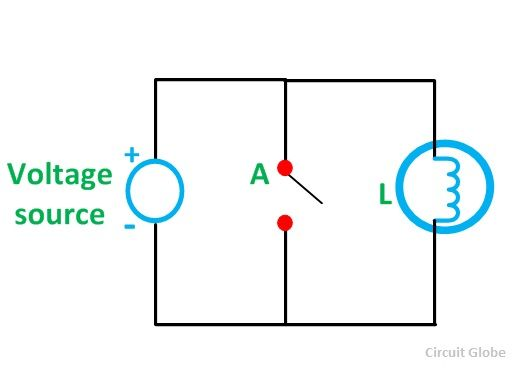
\includegraphics[height=0.5\textheight,width=0.5\textwidth]{figuras/circuito_NOT.jpg} 
 
  &
  \parbox{0.4\linewidth}{\vspace{-4cm} Onde a tabela equivalente é dada por:
  \begin{tabular}{|c|c|}
	\hline
	$\mathbf{A}$ & $\mathbf{\sim A}$ \\
	\hline
	V (ou  \textcolor{red}{1}) & F (ou \textcolor{red}{0}) \\
	\hline
	F (ou \textcolor{red}{0}) & V (ou \textcolor{red}{1})  \\
	\hline
	\end{tabular}
	onde:\\
	V (ou  \textcolor{red}{1}): lâmpada acesa\\
	F (ou \textcolor{red}{0}): lâmpada apagada\\
	\textbf{\textcolor{red}{Conserte o circuito acima !!!}}
  } %% fim do parbox

\end{tabular} 	

\end{frame}


\begin{frame}
\frametitle{A \textbf{conjunção} ou conectivo \textbf{E}  em um circuito elétrico:}

\begin{tabular}{c||c}  
 
 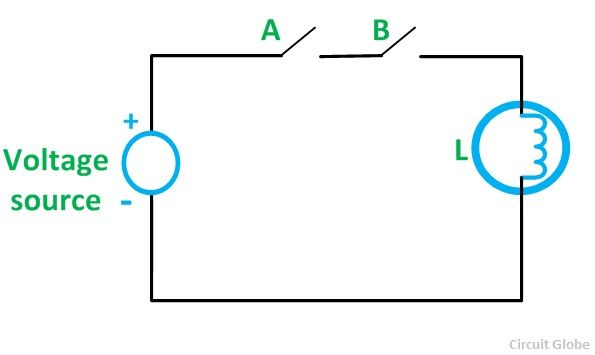
\includegraphics[height=0.5\textheight,width=0.5\textwidth]{figuras/circuito_AND.jpg} 
 
  &
  \parbox{0.4\linewidth}{\vspace{-4cm} Onde a tabela equivalente é dada por:\\
  	\begin{tabular}{|c|c|c|}
	\hline
	$\mathbf{A}$ & $\mathbf{B}$ & $\mathbf{A \wedge B}$ \\
	\hline
	V & V & V \\
	\hline
	V & F & F \\
	\hline
	F & V & F \\
	\hline
	F & F & F \\
	\hline
	\end{tabular}\\
  onde:\\
	V (ou  \textcolor{red}{1}): lâmpada acesa\\
	F (ou \textcolor{red}{0}): lâmpada apagada\\

  } %% fim do parbox

\end{tabular} 	

\end{frame}

\begin{frame}
\frametitle{A \textbf{disjunção} ou conectivo \textbf{OU}  em um circuito elétrico:}

\begin{tabular}{c||c}  
 
 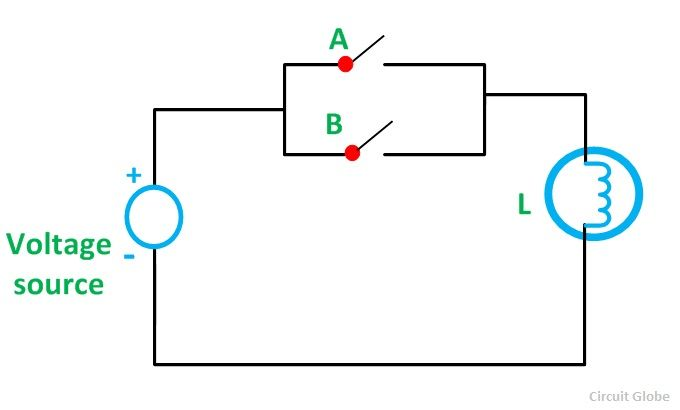
\includegraphics[height=0.5\textheight,width=0.5\textwidth]{figuras/circuito_OR.jpg} 
 
  &
  \parbox{0.4\linewidth}{\vspace{-4cm} Onde a tabela equivalente é dada por:\\
  	\begin{tabular}{|c|c|c|}
	\hline
	$\mathbf{A}$ & $\mathbf{B}$ & $\mathbf{A \vee B}$ \\
	\hline
	V & V & V \\
	\hline
	V & F & V \\
	\hline
	F & V & V \\
	\hline
	F & F & F \\
	\hline
	\end{tabular}\\
  onde:\\
	V (ou  \textcolor{red}{1}): lâmpada acesa \textbf{\textcolor{yellow}{acesa}}\\
	F (ou \textcolor{red}{0}): lâmpada apagada\\

  } %% fim do parbox

\end{tabular} 	

\end{frame}


\begin{frame}
\frametitle{Construa a Tabelas Verdades (TVs) das fórmulas abaixo:}


\begin{block}{Resolva: $\sim A \vee B$}
\begin{center}

	\begin{tabular}{|c|c|c|c|}
	\hline 	\hline
	$\mathbf{A}$ & $\mathbf{B}$ & $\mathbf{\sim A}$ & $\mathbf{\sim A \vee B}$ \\
	\hline
	F & F & V & \\
  \hline
	F & V & V & \\
	\hline
	V & F & F & \\
	\hline
	V & V & F & \\
	\hline 	\hline
	\end{tabular}
\end{center}
  
\begin{itemize}
   \item Para fins de concurso público é algo como: \textit{se A for verdadeiro então B também deverá ser}!
   \item Contudo, se A não for verdade, qualquer coisa serve para B
    \item  Esta fórmula é conhecida como $\sim A \vee B \equiv A \rightarrow B$, leia-se: \textbf{se A  então B}

  \end{itemize}
  \end{block}


\end{frame}


\begin{frame}
\frametitle{Construa a Tabelas Verdades (TVs) das fórmulas abaixo:}


\begin{block}{Resolva: $(\sim A \vee B) \wedge (\sim B \vee A) $}
\begin{center}

	\begin{tabular}{|c|c|c|c|c|c|c|}
	\hline 	\hline
	$\mathbf{A}$ & $\mathbf{B}$ & $\mathbf{\sim A}$ & $X:\mathbf{\sim A \vee B}$ & $\mathbf{\sim B}$ & $Y:\mathbf{\sim B \vee A}$ & $X \wedge Y $ \\
	\hline
	F & F & V &  &  &  &   \\	
	\hline
	F & V & V &  &  &  &   \\
	\hline
	V & F & F &  &  &  &   \\
	\hline
	V & V & F &  &  &  &   \\
	\hline 	\hline
	\end{tabular}
\end{center}
  
\begin{itemize}
   \item Para fins de concurso público é algo como: \textit{se A e B forem iguais então esta fórmula é verdadeira}!
  \item Se A e B forem diferentes, então a expressão é falsa
    \item  Esta fórmula é conhecida como $A \leftrightarrow  B$, leia-se: \textbf{A bi-implica em B}

  \end{itemize}
  \end{block}


\end{frame}




\begin{frame}
\frametitle{Onde tudo isto será usado?}


\begin{block}{Sejam as fórmulas  $A:X=3$ e $B:Y=4$, resolva via TV: }

\begin{itemize}

    \item $X = 3 \vee   Y = 4$
    \item $X = 3 \vee   Y \neq 4$
    \item $X = 3 \wedge Y \neq 4$
    \item $X < 3 \vee   Y = 4$
    \item $X > 3 \wedge Y \neq 4$

\end{itemize}

  \end{block}


\end{frame}



\begin{frame}
\frametitle{Concluindo}


\begin{block}{Isto tudo se relaciona em seguir passos lógicos: }

\begin{itemize}

  \item Como o computador trabalha com \textbf{0}'s e \textbf{1}'s, estas operações de \textbf{V}erdade e \textbf{F}also são análogas
  \pause
    \item O tempo inteiro voce deverá começar a pensar deste modo: $0 = F$ e $1 = V$
      \pause
    \item Claro este princípio não serve para vida!
      \pause
    \item Mas, aqui para o curso sim!
      \pause
    \item Boa sorte!

\end{itemize}

  \end{block}


\end{frame}











\end{document}
